\graphicspath{ {../../images/} }
\usetikzlibrary{
  calc,
  decorations.pathreplacing,
  decorations.pathmorphing,
  shapes,
  positioning,
  patterns,
  shadows.blur,
  external,
  overlay-beamer-styles}
\usepackage{pifont}

\title{ITC8280 Fundamentals of Cryptography}
\subtitle{Block ciphers \& AES}
\date{\today}
\author{Taaniel Kraavi}
\institute%
{%
  \textit{School of Information Technologies}\\
  \textit{Tallinn University of Technology}
}

\begin{document}
\begin{frame}
  \titlepage
\end{frame}

\begin{frame}{Block ciphers}
  \begin{center}
  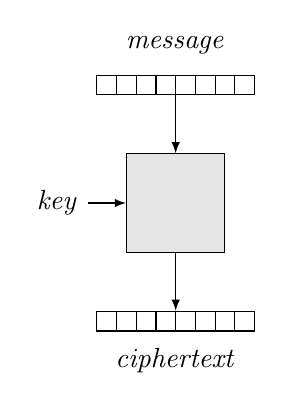
\begin{tikzpicture}
    %\node (f) at ($(2.5cm,0)$) [minimum size=1.25cm,rounded corners=1ex,fill=red!20,draw] {$\ENC$};
    \node (f) at ($(2.5cm,0)$) [minimum size=1.25cm,fill=gray!20,draw] {$\ENC$};
    \node (m) [above of=f, node distance=2cm] {\textit{message}};
    \node (k) [left of=f, node distance=1.5cm] {\textit{key}};
    \node (c) [below of=f, node distance=2cm] {\textit{ciphertext}};

    \node[rectangle, draw, text width=2cm, text height=0.25cm] (mbox)
    [
      below of=m,
      node distance=0.5cm,
      inner sep=0,
      %outer sep=0.1cm,
      path picture={\draw[step=0.25]
        (path picture bounding box.north west)
        grid
        (path picture bounding box.south east);
      }] {};
    \node[rectangle, draw, text width=2cm, text height=0.25cm] (cbox)
    [
      above of=c,
      node distance=0.5cm,
      inner sep=0,
      %outer sep=0.1cm,
      path picture={\draw[step=0.25]
        (path picture bounding box.north west)
        grid
        (path picture bounding box.south east);
    }] {};

    \draw[-latex] (mbox) -- (f);
    \draw[-latex] (k) -- (f);
    \draw[-latex] (f) -- (cbox);
  \end{tikzpicture}
  \hspace*{2cm}
  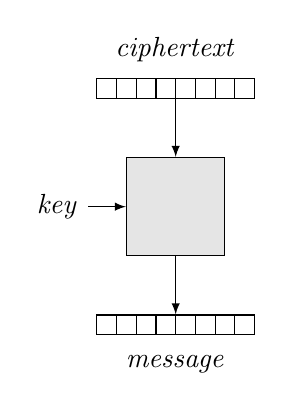
\begin{tikzpicture}
    %\node (f) at ($(2.5cm,0)$) [minimum size=1.25cm,rounded corners=1ex,fill=red!20,draw] {$\ENC$};
    \node (f) at ($(2.5cm,0)$) [minimum size=1.25cm,fill=gray!20,draw] {$\DEC$};
    \node (c) [above of=f, node distance=2cm] {\textit{ciphertext}};
    \node (k) [left of=f, node distance=1.5cm] {\textit{key}};
    \node (m) [below of=f, node distance=2cm] {\textit{message}};

    \node[rectangle, draw, text width=2cm, text height=0.25cm] (cbox)
    [
      below of=c,
      node distance=0.5cm,
      inner sep=0,
      %outer sep=0.1cm,
      path picture={\draw[step=0.25]
        (path picture bounding box.north west)
        grid
        (path picture bounding box.south east);
      }] {};
    \node[rectangle, draw, text width=2cm, text height=0.25cm] (mbox)
    [
      above of=m,
      node distance=0.5cm,
      inner sep=0,
      %outer sep=0.1cm,
      path picture={\draw[step=0.25]
        (path picture bounding box.north west)
        grid
        (path picture bounding box.south east);
    }] {};

    \draw[-latex] (cbox) -- (f);
    \draw[-latex] (k) -- (f);
    \draw[-latex] (f) -- (mbox);
  \end{tikzpicture}
  \end{center}

  \pause
  Block ciphers are deterministic and operate on fixed-length \emph{blocks}.
  \begin{itemize}[<+(1)->]
    \item $E_K(\cdot) \defeq E(K, \cdot) : \{0, 1\}^s \times \{0, 1\}^n \to \{0, 1\}^n$
  \end{itemize}
\end{frame}

\begin{frame}{Block cipher versatility}
  Built using block ciphers:
  \begin{itemize}[<+(1)->]
    \item Stream ciphers
    \item CSPRNGs
    \item Cryptographic hash functions
    \item Secure PRPs (pseudo-random permutations)
    \item Message authentication codes (MACs) \& AE
  \end{itemize}
\end{frame}

\begin{frame}{Modes of operation}
  \pause
  \emph{Modes of operation} are used to extend operations to data larger than a block.
  \begin{itemize}[<+(1)->]
    \item Some modes also provide authenticity
  \end{itemize}

  \vspace*{0.5em}

  \pause
  Examples:
  \begin{columns}
    \begin{column}{0.4\textwidth}
      \begin{itemize}[<+(1)->]
        \item ECB (NB! danger-zone)
        \item CBC
      \end{itemize}
    \end{column}
    \begin{column}{0.5\textwidth}
      \begin{itemize}[<+(1)->]
        \item CTR
        \item GCM (authenticated encryption)
      \end{itemize}
    \end{column}
  \end{columns}

  \vspace*{1em}

  \pause
  Important:
  \begin{itemize}[<+(1)->]
    \item A secure cipher with an insecure mode is insecure!
    \item Pick the right mode for the right task!
  \end{itemize}  
\end{frame}

\begin{frame}{Electronic Codebook (ECB) mode}
  \begin{center}
  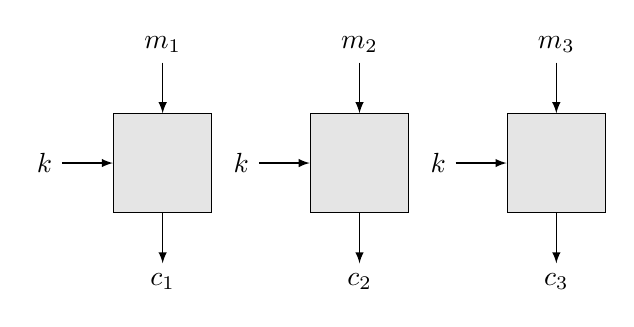
\begin{tikzpicture}
    \foreach \x in {1, 2, 3} {
      \node (f\x) at ($\x*(2.5cm,0)$) [minimum size=1.25cm,fill=gray!20,draw] {$\ENC$};
      \node (m\x) [above of=f\x, node distance=1.5cm] {$m_\x$};
      \node (k\x) [left of=f\x, node distance=1.5cm] {$k$};
      \node (c\x) [below of=f\x, node distance=1.5cm] {$c_\x$};

      \draw[-latex] (m\x) -- (f\x);
      \draw[-latex] (k\x) -- (f\x);
      \draw[-latex] (f\x) -- (c\x);
    }
  \end{tikzpicture}
  \end{center}

  \pause
  Do not use, \emph{ever}\textsuperscript{*}

  \pause
  A building block for
  \begin{itemize}[<+->]
    \item more complex modes
    \item other cryptographic constructions
  \end{itemize}
\end{frame}

\begin{frame}{ECB Tux}
  \begin{columns}
    \begin{column}{0.5\textwidth}
      \begin{center}
        \includegraphics[width=150px]{tux}
      \end{center}
    \end{column}
    \begin{column}{0.5\textwidth}
      \pause
      \begin{center}
        \includegraphics[width=150px]{tux_ecb}
      \end{center}
    \end{column}
  \end{columns}
\end{frame}

\begin{frame}{Core tenet of encryption}
  \begin{center}
    IND-CPA requires randomised encryption!

    \vspace*{2em}

    \pause
    Ephemeral random values are necessary, but not sufficient for IND-CPA.
  \end{center}
\end{frame}

\begin{frame}{Initialisation Vector (IV)}
  \begin{center}
  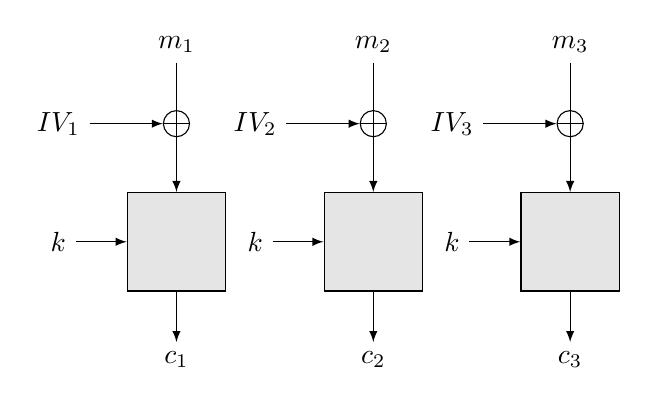
\begin{tikzpicture}
    \foreach \x in {1, 2, 3} {
      \node (f\x) at ($\x*(2.5cm,0)$) [minimum size=1.25cm,fill=gray!20,draw] {$\ENC$};
      \node (p\x) [above of=f\x, node distance=1.5cm, circle, draw] {};
      \node (m\x) [above of=p\x, node distance=1cm] {$m_\x$};
      \node (k\x) [left of=f\x, node distance=1.5cm] {$k$};
      \node (c\x) [below of=f\x, node distance=1.5cm] {$c_\x$};

      \draw[-] (p\x.east) -- (p\x.west);

      \draw[-latex] (m\x) -- (f\x);
      \draw[-latex] (k\x) -- (f\x);
      \draw[-latex] (f\x) -- (c\x);

      \node (iv\x) [left of=p\x, node distance=1.5cm] {$IV_\x$};
      \draw[-latex] (iv\x) -- (p\x);
    }
  \end{tikzpicture}
  \end{center}

  \begin{itemize}[<+(1)->]
    \item Different ways to apply the IV (XOR on the figure)
    \item Do not reuse (under the same key)
    \item Not secret: sent with the ciphertext
  \end{itemize}
\end{frame}

\begin{frame}{Cipher Block Chaining (CBC) mode}
  \begin{center}
  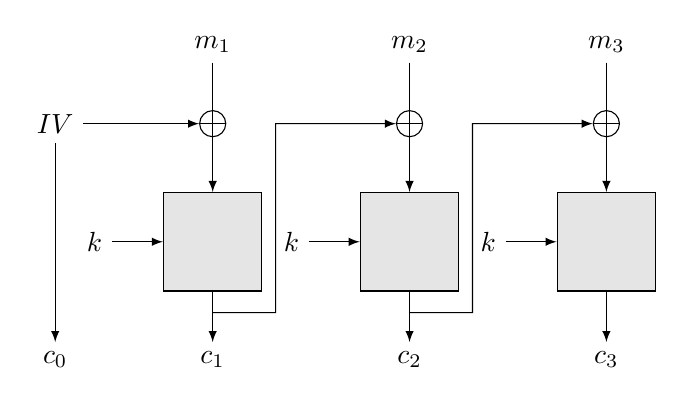
\begin{tikzpicture}
    \foreach \x in {1, 2, 3} {
      \node (f\x) at ($\x*(2.5cm,0)$) [minimum size=1.25cm,fill=gray!20,draw] {$\ENC$};
      \node (p\x) [above of=f\x, node distance=1.5cm, circle, draw] {};
      \node (m\x) [above of=p\x, node distance=1cm] {$m_\x$};
      \node (k\x) [left of=f\x, node distance=1.5cm] {$k$};
      \node (c\x) [below of=f\x, node distance=1.5cm] {$c_\x$};

      \draw[-] (p\x.east) -- (p\x.west);

      \draw[-latex] (m\x) -- (f\x);
      \draw[-latex] (k\x) -- (f\x);
      \draw[-latex] (f\x) -- (c\x);
    }

    \node (iv) [left of=p1, node distance=2cm] {$IV$};
    \draw[-latex] (iv) -- (p1);

    \node (c0) [left of=c1, node distance=2cm] {$c_0$};
    \draw[-latex] (iv) -- (c0);

    \foreach \x in {1, 2} {
        \draw[-latex] ($(c\x) + (0,0.6cm)$) -| +(0.8cm,2.4cm) -- ($(p\the\numexpr\x+1\relax.west)$);
    }
  \end{tikzpicture}
  \end{center}

  \begin{columns}
    \begin{column}{0.5\textwidth}
      \begin{itemize}[<+(1)->]
        \item Serial encryption
        \item Parallel decryption
        \item Pre-encryption change propagation
    \end{itemize}
    \end{column}
    \begin{column}{0.5\textwidth}
      \pause
      \begin{block}{Note}
        Not security properties!
      \end{block}
    \end{column}
  \end{columns}
\end{frame}

\begin{frame}{CBC Tux}
  \begin{columns}
    \begin{column}{0.5\textwidth}
      \begin{center}
        \includegraphics[width=150px]{tux}
      \end{center}
    \end{column}
    \begin{column}{0.5\textwidth}
      \pause
      \begin{center}
        \includegraphics[width=150px]{tux_secure}
      \end{center}
    \end{column}
  \end{columns}
\end{frame}

\begin{frame}
  \frametitle{Counter (CTR) mode}

  \begin{center}
  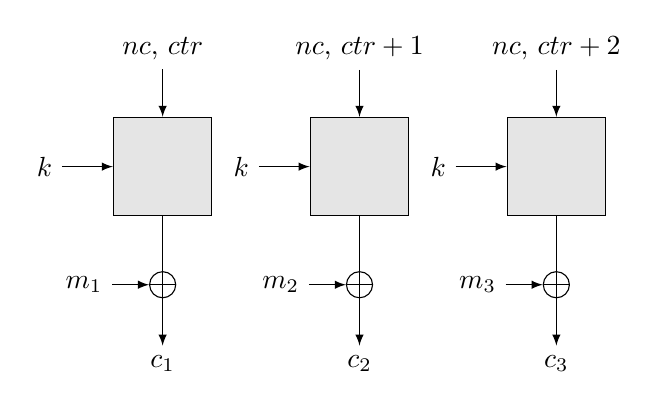
\begin{tikzpicture}
    \node (f1) at ($(2.5cm,0)$) [minimum size=1.25cm,fill=gray!20,draw] {$\ENC$};
    \node (n1) [above of=f1, node distance=1.5cm] {$nc$, $ctr$};
    \node (k1) [left of=f1, node distance=1.5cm] {$k$};
    \node (c1) [below of=f1, node distance=2.5cm] {$c_1$};
    \node (p1) [below of=f1, node distance=1.5cm, circle, draw] {};
    \node (m1) [left of=p1, node distance=1cm] {$m_1$};

    \draw[-] (p1.east) -- (p1.west);

    \draw[-latex] (n1) -- (f1);
    \draw[-latex] (m1) -- (p1);
    \draw[-latex] (k1) -- (f1);
    \draw[-latex] (f1) -- (c1);

    \foreach \x in {2, 3} {
      \node (f\x) at ($\x*(2.5cm,0)$) [minimum size=1.25cm,fill=gray!20,draw] {$\ENC$};
      \node (n\x) [above of=f\x, node distance=1.5cm] {$nc$, $ctr+\the\numexpr\x-1$};
      \node (k\x) [left of=f\x, node distance=1.5cm] {$k$};
      \node (c\x) [below of=f\x, node distance=2.5cm] {$c_\x$};
      \node (p\x) [below of=f\x, node distance=1.5cm, circle, draw] {};
      \node (m\x) [left of=p\x, node distance=1cm] {$m_\x$};

      \draw[-] (p\x.east) -- (p\x.west);

      \draw[-latex] (n\x) -- (f\x);
      \draw[-latex] (m\x) -- (p\x);
      \draw[-latex] (k\x) -- (f\x);
      \draw[-latex] (f\x) -- (c\x);
    }
  \end{tikzpicture}
  \end{center}

  \begin{itemize}[<+(1)->]
    \item Operates as a stream cipher
    \item Counter combined using an \emph{invertible} operation, e.g. $\oplus$, $+$, $||$
    \item $||$ preferred due to counter pitfalls (e.g. with non-random nonces)
  \end{itemize}
\end{frame}

\begin{frame}{Authenticated encryption (AE)}
  \begin{block}{Note}
    We will cover data authentication \& integrity in a later lecture.
  \end{block}

  \vspace*{0.5em}
  
  AE provides confidentiality \& authenticity.
  \begin{itemize}[<+(1)->]
    \item Authenticity and integrity provided by the \emph{authentication tag}
    \item If tag verification fails, do not decrypt the ciphertext
    \item Do not use\textsuperscript{*} unauthenticated encryption! \hspace{1em} {\scriptsize\textsuperscript{*}without a very good reason}
  \end{itemize}

  \vspace*{1em}

  \pause
  Authenticated encryption with associated data (AEAD):
  \begin{itemize}[<+(1)->]
    \item Additional associated data AAD: the \emph{header}
    \item Authenticated, but not confidential
  \end{itemize}
\end{frame}

\begin{frame}
  \frametitle{Galois/Counter (GCM) mode}

  You do not need to remember this schema!
  \begin{center}
    \url{https://csrc.nist.rip/groups/ST/toolkit/BCM/documents/proposedmodes/gcm/gcm-spec.pdf\#page=8}
  \end{center}
  \pause
  However, you should understand what it does and why it is useful.
\end{frame}

\begin{frame}{Pitfalls of GCM}
  In GCM-mode, nonce reuse enables the \enquote{forbidden attack}:
  \begin{itemize}[<+(1)->]
    \item practical attack (real-world applicable)
    \item enables authentication key recovery $\implies$ data forgery
  \end{itemize}

  \pause
  How can we protect against nonce reuse?

  \pause
  SIV mode:
  \begin{itemize}[<+->]
    \item Synthetic initialization vector
    \item \href{https://datatracker.ietf.org/doc/html/rfc5297}{RFC 5297}
    \item Example: AES-GCM-SIV (\href{https://datatracker.ietf.org/doc/html/rfc8452}{RFC 8452})
  \end{itemize}
\end{frame}

\begin{frame}{Padding messages}
  \begin{columns}
    \begin{column}{0.5\textwidth}
      \begin{itemize}[<+(1)->]
        \item Zero padding\\
        \texttt{1a 1a 1a 1a 1a 00 00 00}
        \item ISO/IEC 7816-4\\
        \texttt{1a 1a 1a 1a 1a 80 00 00}
        \item PKCS\#5 and PKCS\#7 (most common)\\
        \texttt{1a 1a 1a 1a 1a 03 03 03}\\
        \texttt{1a 1a 1a 05 05 05 05 05}
      \end{itemize}
    \end{column}
    \begin{column}{0.5\textwidth}
      \begin{itemize}[<+(1)->]
        \item ANSI X9.23 (withdrawn)\\
        \texttt{1a 1a 1a 1a 1a 00 00 03}
        \item ISO 10126 (withdrawn)\\
        \texttt{1a 1a 1a 1a 1a 81 A6 03}
      \end{itemize}
    \end{column}
  \end{columns}

  \vspace*{1em}

  \pause
  In non-streaming modes, padding should always be added for unambiguity!
  \begin{itemize}[<+(1)->]
    \item If the message is block-aligned, add a full padding block
    \item NOT intended for randomisation: that is the IV's role
  \end{itemize}
\end{frame}

\begin{frame}{Block-size \& key size}
  A block cipher may have different parameters for the \enquote{same} cipher.

  \pause
  Block size:
  \begin{itemize}
    \item The number of bits in a block
    \pause
    \item Typically 128, with demand for 256 bits
    \item Historically 64 bits (bad due to increased collision risks)
  \end{itemize}

  \pause
  Key length:
  \begin{itemize}
    \item Usually tied to the \enquote{strength} of the cipher
    \pause
    \item Typical values are: 128, 192, 256 bits
    \item 128 bits is the strict minimum!
  \end{itemize}

  \pause
  More complex parameters exist, but are not usually for the user to tune.
\end{frame}

\begin{frame}{Security level}
  \pause
  The \emph{security level} is a measure of the \enquote{strength} that a cryptographic primitive achieves.

  \begin{itemize}[<+(1)->]
    \item Often called \emph{bits of security}
    \item $n$-bits of security: $2^n$ operations to break (typical definition)
    \item Strength measured differently for different primitives!
    \par
    \begin{itemize}
      \item Consult authoritative sources (e.g. NIST, ANSSI, BSI)
      \item Not always clear cut
    \end{itemize}
    \par
    \item For symmetric cryptosystems:
    \begin{itemize}
      \item classical strength = key size 
      \item quantum resistance = half of the key size
    \end{itemize}
  \end{itemize}
\end{frame}

\begin{frame}{Cryptographic break}
  In terms of the \enquote{raw} security level:
  \begin{itemize}[<+(1)->]
    \item Computational break: attack with lower complexity than the claimed level
    \item Not all \emph{breaks} are practical
    \item Theoretical breaks can still be useful
    \item Historically accepted minimum security levels: $2^{80}$, later $2^{112}$
    \item Modern minimum required security level: 128 bits
  \end{itemize}
\end{frame}

\begin{frame}{Some ciphers}
  Some well-known ciphers include
  \begin{itemize}[<+(1)->]
    \item[\ding{55}] DES (Data Encryption Standard): belongs in a museum, weak!
    \item[\ding{55}] 3DES: deprecated
    \item[\ding{51}] Twofish: successor to the insecure Blowfish
    \item[\ding{51}] RC6: used to be patented, successor to RC5
    \item[\ding{51}] Camellia, Serpent, ARIA, \dots
    \item[\ding{51}]AES (Advanced Encryption Standard): sometimes called the \enquote{gold standard}
  \end{itemize}

  \vspace*{1em}

  \pause
  Block ciphers seem (and are) more \enquote{popular}.
  \begin{itemize}[<+(1)->]
    \item historical reasons, e.g. perception (RC4) \& standardisation
    \item security analysis is \enquote{easier}
    \item versatility
  \end{itemize}
\end{frame}

\begin{frame}{AES}
  Advanced Encryption Standard
  \pause
  \begin{itemize}
    \item Originally called Rijndael
    \item Standardised by NIST in 2001 (\href{https://csrc.nist.gov/pubs/fips/197/final}{FIPS 197})
    \item Later standardised by ISO (\href{https://www.iso.org/standard/54531.html}{ISO/IEC 18033-3:2010})
    \item Superseded the Data Encryption Standard (DES)
  \end{itemize}

  \pause
  Practical info:
  \begin{itemize}[<+(1)->]
    \item Block size: 128 bits
    \item \href{https://csrc.nist.gov/pubs/sp/800/197/iprd}{NIST SP 800-197}: work on 256-bit block AES (in progress)
    \item Key sizes: 128, 192, 256 bits
  \end{itemize}
\end{frame}

\begin{frame}{Attacks on AES}
  No practical attack is known against the AES cipher (when correctly implemented).

  \begin{itemize}[<+(1)->]
    \item Best known key recovery attack: $\sim 2^{126}$ operations (not practical)
    \item AES-256 is considered \emph{quantum resistant} (128 bits of security)
    \item AES-128 and AES-192 are not considered sufficient for quantum safety
    \item Implementation dangers: side channel attacks
    \par
    \begin{itemize}
      \item Hardware implementations \emph{should} be protected against cache timing attacks
    \end{itemize}
  \end{itemize}

  \pause
  Pick the implementation carefully!
\end{frame}

\begin{frame}{Symmetric encryption recap}
  Use AE(AD) constructions whenever possible!
  \begin{itemize}[<+(1)->]
    \item Do not reuse nonces: breaks confidentiality
    
    \vspace*{0.5em}

    \item AES-GCM should be your default choice
    \begin{itemize}
      \item 128/192/256-bit keys, 96-bit nonce (standard)
      \item Brittle: nonce reuse enables universal forgeries
      \item May be slow without AES hardware support
    \end{itemize}

    \vspace*{0.5em}

    \item ChaCha20-Poly1305 is the primary alternative
    \begin{itemize}[<+(1)->]
      \item Fast without hardware support
      \item 256-bit key, 96-bit nonce (192-bit XChaCha20)
      \item Not standardised by NIST (not FIPS compliant)
    \end{itemize}
  \end{itemize}
\end{frame}

\begin{frame}{Data limits}
  AES-GCM:
  \begin{itemize}[<+(1)->]
    \item Message length limit: $2^{32} - 2$ blocks $\approx 64$ GiB
    \item Re-keying needed after $2^{32}$ encryptions (distinct IVs) \href{https://csrc.nist.gov/pubs/sp/800/38/d/final}{[SP 800-38D \S 8.3]}
  \end{itemize}

  \vspace*{0.5em}

  \pause
  ChaCha20-Poly1305:
  \begin{itemize}[<+(1)->]
    \item 96-bit nonce message length limit: $\approx 256$ GiB \href{https://datatracker.ietf.org/doc/html/rfc8439\#section-2.8}{[RFC 8439]}
    \item Re-keying? Some theoretical bounds, but no concrete recommendations
  \end{itemize}

  \vspace*{0.5em}

  \pause
  Nonce/IV reuse may be catastrophic (under the same key)!
  \begin{itemize}[<+(1)->]
    \item Nonce/IV space may need to be partitioned in multi-sender cases
    \item Re-key well before the \enquote{trouble} bounds
  \end{itemize}
\end{frame}

\begin{frame}{IND-CCA1: lunchtime attack (non-adaptive)}
  \begin{figure}
    \centering
    \begin{tikzpicture}[
      scale=0.9, transform shape,
      Squiggly/.style={
        decorate,
        decoration={snake, segment length=4, amplitude=0.9},
      },
      arrowlabel/.style={
        midway,
        fill=bg,
        inner sep=2pt,
        rounded corners=1pt,
      },
      divider/.style={
        dotted,
        thick
      },
      challengeline/.style={
        thick,
        gray!70,
      },
      phaselabel/.style={
        anchor=west,
        font=\footnotesize
      }]

      \draw[rounded corners,thick,fill=blue!50] (5, 0) rectangle ++(3, -5);
      \draw[rounded corners,thick,fill=red!85]  (0, 0) rectangle ++(1, -5);

      \node (P) at (6.5, 0.5) {Challenger};
      \node (K) at (0.5, 0.5) {$\AD$};

      \draw[->,thick,visible on=<3->] (1, -1.5) -- (5, -1.5)
        node[arrowlabel] {$m_i \lor c_i$};
      \draw[<-,thick,visible on=<3->] (1, -2)   -- (5, -2)
        node[arrowlabel] {$\ENC_k(m_i) \lor \DEC_k(c_i)$};

      \node[visible on=<2->] at (6.5, -0.5) {$k \gets \GEN()$};
      \node[visible on=<4->] at (6.5, -3.25) {$b \getsu \{0, 1\}$};
      \node[visible on=<4->] at (6.5, -3.75) {$C \gets \ENC_k(M_b)$};

      \draw[->,thick,visible on=<4->] (1, -3) -- (5, -3) node[arrowlabel] {$M_0, M_1$};
      \draw[<-,thick,visible on=<4->] (1, -4) -- (5, -4) node[arrowlabel] {$C$};

      \draw[->,thick,visible on=<5->] (0.5, -5) decorate[Squiggly]{ -- (0.5, -5.36) };
      \node[visible on=<5->] at (0.5, -5.6) {$b'$};

      \def\phasex{8.5}

      \draw[divider,visible on=<3->] (-1, -1) -- (9, -1)
        node[above=2pt, anchor=west, fill=bg, inner sep=2pt] {};
      \node[phaselabel,visible on=<2->] at (\phasex, -0.5) {Setup};

      \draw[divider,visible on=<4->] (-1, -2.5) -- (9, -2.5)
        node[above=2pt, anchor=west, fill=bg, inner sep=2pt] {};
      \node[phaselabel,visible on=<3->] at (\phasex, -1.75) {Phase 1};

      \draw[divider,visible on=<5->] (-1, -4.5) -- (9, -4.5)
        node[below=2pt, anchor=west, fill=bg, inner sep=2pt] {};
      \node[phaselabel,visible on=<4->] at (\phasex, -3.5) {Challenge};

      \draw[
        decorate,
        decoration={brace, mirror, amplitude=6pt},
        visible on=<3->
      ] (-0.1, -1.1) -- (-0.1, -2.4) {};
      \node[anchor=east,font=\footnotesize,visible on=<3->] at (-0.3, -1.75) {loop};
    \end{tikzpicture}
  \end{figure}

  \visible<6->{NB! We assume that (challenge) messages are of equal length.}
\end{frame}

\begin{frame}{IND-CCA2: adaptive}
  The adversary can submit new queries after receiving the challenge.

  \pause
  \begin{figure}
    \centering
    \begin{tikzpicture}[
      scale=0.9, transform shape,
      Squiggly/.style={
        decorate,
        decoration={snake, segment length=4, amplitude=0.9},
      },
      arrowlabel/.style={
        midway,
        fill=bg,
        inner sep=2pt,
        rounded corners=1pt,
      },
      divider/.style={
        dotted,
        thick
      },
      challengeline/.style={
        thick,
        gray!70,
      },
      phaselabel/.style={
        anchor=west,
        font=\footnotesize
      }]

      \draw[rounded corners,thick,fill=blue!50] (5, 0) rectangle ++(3, -5);
      \draw[rounded corners,thick,fill=red!85]  (0, 0) rectangle ++(1, -5);

      \node[visible on=<2->] at (0.5, -0.5) {$\vdots$};
      \node[visible on=<2->] at (6.5, -0.5) {$\vdots$};

      \node[visible on=<3->] at (6.5, -1.75) {$b \getsu \{0, 1\}$};
      \node[visible on=<3->] at (6.5, -2.25) {$C \gets \ENC_k(M_b)$};

      \draw[->,thick,visible on=<3->] (1, -1.5) -- (5, -1.5) node[arrowlabel] {$M_0, M_1$};
      \draw[<-,thick,visible on=<3->] (1, -2.5) -- (5, -2.5) node[arrowlabel] {$C$};

      \node[visible on=<4->] at (6.5, -3.75) {$\mathsf{Abort\ if\ } c_j = C$};

      \draw[->,thick,visible on=<4->] (1, -3.5) -- (5, -3.5)
        node[arrowlabel] {$m_j \lor c_j$};
      \draw[<-,thick,visible on=<4->] (1, -4)   -- (5, -4)
        node[arrowlabel] {$\ENC_k(m_j) \lor \DEC_k(c_j)$};

      \draw[->,thick,visible on=<5->] (0.5, -5) decorate[Squiggly]{ -- (0.5, -5.36) };
      \node[visible on=<5->] at (0.5, -5.6) {$b'$};

      \def\phasex{8.5}

      \draw[divider,visible on=<3->] (-1, -1) -- (9, -1)
        node[above=2pt, anchor=west, fill=bg, inner sep=2pt] {};
      \node[phaselabel,visible on=<2->,align=left] at (\phasex, -0.5) {Setup +\\Phase 1};

      \draw[divider,visible on=<4->] (-1, -3) -- (9, -3)
        node[below=2pt, anchor=west, fill=bg, inner sep=2pt] {};
      \node[phaselabel,visible on=<3->] at (\phasex, -2) {Challenge};

      \draw[divider,visible on=<5->] (-1, -4.5) -- (9, -4.5)
        node[below=2pt, anchor=west, fill=bg, inner sep=2pt] {};
      \node[phaselabel,visible on=<4->] at (\phasex, -3.75) {Phase 2};

      \draw[
        decorate,
        decoration={brace, mirror, amplitude=6pt},
        visible on=<4->
      ] (-0.1, -3.1) -- (-0.1, -4.4) {};
      \node[anchor=east,font=\footnotesize,visible on=<4->] at (-0.3, -3.75) {loop};
    \end{tikzpicture}
  \end{figure}
\end{frame}

\begin{frame}{Disk encryption (brief)}
  Disk encryption has some tricky requirements.

  \pause
  How to do it with CBC?
  \begin{itemize}[<+(1)->]
    \item Encrypt each (logical) sector
    \item Use sector number as IV
    \item ESSIV mode improves it a little (SN + key hash)
    \item No integrity!
  \end{itemize}

  \pause
  Name dropping:
  \begin{itemize}[<+(1)->]
    \item XTS-AES
    \item Google Adiantum (cipher composition)
  \end{itemize}
\end{frame}

\begin{frame}{Keys and passwords}
  \pause
  A human-generated password typically has low \emph{entropy}, i.e. not random enough.

  \pause
  Key derivation functions (more next week):
  \begin{itemize}[<+(1)->]
    \item Derive secret keys from a secret value
    \item \enquote{Stretch} (and strengthen) secrets
  \end{itemize}

  \vspace*{1em}

  \pause
  E.g. disk encryption key wrapping:
  \begin{itemize}[<+(1)->]
    \item Generate random disk encryption key (DEK)
    \item Derive encryption key from use-provided password (KEK)
    \item Encrypt DEK with KEK
  \end{itemize}
\end{frame}

\end{document}
